%%%%%%%%%%%%%%%%%%%%%%%%%%%%%%%%%%%%%%%%%%%%%%%%%%%%%%%%%%%%%%%%%%%%%%%%%%%%%%%%
%% Plantilla de memoria en LaTeX para la ETSIT - Universidad Rey Juan Carlos
%%
%% Por Gregorio Robles <grex arroba gsyc.urjc.es>
%%     Grupo de Sistemas y Comunicaciones
%%     Escuela Técnica Superior de Ingenieros de Telecomunicación
%%     Universidad Rey Juan Carlos
%% (muchas ideas tomadas de Internet, colegas del GSyC, antiguos alumnos...
%%  etc. Muchas gracias a todos)
%%
%% La última versión de esta plantilla está siempre disponible en:
%%     https://github.com/gregoriorobles/plantilla-memoria
%%
%% Para obtener PDF, ejecuta en la shell:
%%   make
%% (las imágenes deben ir en PNG o JPG)

%%%%%%%%%%%%%%%%%%%%%%%%%%%%%%%%%%%%%%%%%%%%%%%%%%%%%%%%%%%%%%%%%%%%%%%%%%%%%%%%

\documentclass[a4paper, 12pt]{book}
%\usepackage[T1]{fontenc}

\usepackage[a4paper, left=2.5cm, right=2.5cm, top=3cm, bottom=3cm]{geometry}
\usepackage{times}
\usepackage[utf8]{inputenc}
\usepackage[spanish]{babel} % Comenta esta línea si tu memoria es en inglés
\usepackage{url}
%\usepackage[dvipdfm]{graphicx}
\usepackage{graphicx}
\usepackage{float}  %% H para posicionar figuras
\usepackage[breaklinks=true]{hyperref}
\usepackage[nottoc, notlot, notlof, notindex]{tocbibind} %% Opciones de índice
\usepackage{latexsym}  %% Logo LaTeX
\usepackage{amsmath, amsthm}


\title{Memoria del Proyecto}
\author{Rosa Cristina Ruiz Rivas}

\renewcommand{\baselinestretch}{1.5}  %% Interlineado

\begin{document}

\renewcommand{\refname}{Bibliografía}  %% Renombrando
\renewcommand{\appendixname}{Apéndice}

%%%%%%%%%%%%%%%%%%%%%%%%%%%%%%%%%%%%%%%%%%%%%%%%%%%%%%%%%%%%%%%%%%%%%%%%%%%%%%%%
% PORTADA

\begin{titlepage}
\begin{center}
\includegraphics[scale=0.8]{img/URJ_logo_Color_POS.png}

\vspace{1.75cm}

\Large
DOBLE GRADO EN INGENIERÍA EN SISTEMAS DE TELECOMUNICACIÓN Y ADMINISTRACIÓN Y DIRECCIÓN DE EMPRESAS 

\vspace{0.4cm}

\large
Curso Académico 2021/2022

\vspace{0.8cm}

Trabajo Fin de Grado

\vspace{2.5cm}

\LARGE
ANÁLISIS DE DATOS DEL PENSAMIENTO COMPUTACIONAL DE PROYECTOS DE SCRATCH Y SNAP!

\vspace{3cm} 

\large
Autora : Rosa Cristina Ruiz Rivas \\
Tutor : Dr. Gregorio Robles Martínez
\end{center}
\end{titlepage}

\newpage
\mbox{}
\thispagestyle{empty} % para que no se numere esta pagina


%%%%%%%%%%%%%%%%%%%%%%%%%%%%%%%%%%%%%%%%%%%%%%%%%%%%%%%%%%%%%%%%%%%%%%%%%%%%%%%%
%%%% Para firmar
\clearpage
\pagenumbering{gobble}
\chapter*{}

\vspace{-4cm}
\begin{center}
\LARGE
\textbf{Trabajo Fin de Grado}

\vspace{1cm}
\large
Análisis de Datos del Pensamiento Computacional de Proyectos de Scratch y Snap!

\vspace{1cm}
\large
\textbf{Autora :} Rosa Cristina Ruiz Rivas \\
\textbf{Tutor :} Dr. Gregorio Robles Martínez

\end{center}

\vspace{1cm}
La defensa del presente Proyecto Fin de Grado se realizó el día \qquad$\;\,$ de \qquad\qquad\qquad\qquad \newline de 2022, siendo calificada por el siguiente tribunal:


\vspace{0.5cm}
\textbf{Presidente:}

\vspace{1.2cm}
\textbf{Secretario:}

\vspace{1.2cm}
\textbf{Vocal:}


\vspace{1.2cm}
y habiendo obtenido la siguiente calificación:

\vspace{1cm}
\textbf{Calificación:}


\vspace{1cm}
\begin{flushright}
Fuenlabrada, a \qquad$\;\,$ de \qquad\qquad\qquad\qquad de 2022
\end{flushright}

%%%%%%%%%%%%%%%%%%%%%%%%%%%%%%%%%%%%%%%%%%%%%%%%%%%%%%%%%%%%%%%%%%%%%%%%%%%%%%%%
%%%% Dedicatoria

\chapter*{}
\pagenumbering{Roman} % para comenzar la numeracion de paginas en numeros romanos
\begin{flushright}
\textit{Dedicado a \\
mi familia / mi abuelo / mi abuela}
\end{flushright}

%%%%%%%%%%%%%%%%%%%%%%%%%%%%%%%%%%%%%%%%%%%%%%%%%%%%%%%%%%%%%%%%%%%%%%%%%%%%%%%%
%%%% Agradecimientos

\chapter*{Agradecimientos}
%\addcontentsline{toc}{chapter}{Agradecimientos} % si queremos que aparezca en el índice
\markboth{AGRADECIMIENTOS}{AGRADECIMIENTOS} % encabezado 

Aquí vienen los agradecimientos\ldots Aunque está bien acordarse de la pareja, no hay que olvidarse de dar las gracias a tu madre, que aunque a veces no lo parezca disfrutará tanto de tus logros como tú\ldots 
Además, la pareja quizás no sea para siempre, pero tu madre sí.

%%%%%%%%%%%%%%%%%%%%%%%%%%%%%%%%%%%%%%%%%%%%%%%%%%%%%%%%%%%%%%%%%%%%%%%%%%%%%%%%
%%%% Resumen

\chapter*{Resumen}
%\addcontentsline{toc}{chapter}{Resumen} % si queremos que aparezca en el índice
\markboth{RESUMEN}{RESUMEN} % encabezado

Aquí viene un resumen del proyecto.
Ha de constar de tres o cuatro párrafos, donde se presente de manera clara y concisa de qué va el proyecto. 
Han de quedar respondidas las siguientes preguntas:

\begin{itemize}
  \item ¿De qué va este proyecto? ¿Cuál es su objetivo principal?
  \item ¿Cómo se ha realizado? ¿Qué tecnologías están involucradas?
  \item ¿En qué contexto se ha realizado el proyecto? ¿Es un proyecto dentro de un marco general?
\end{itemize}

Lo mejor es escribir el resumen al final.

%%%%%%%%%%%%%%%%%%%%%%%%%%%%%%%%%%%%%%%%%%%%%%%%%%%%%%%%%%%%%%%%%%%%%%%%%%%%%%%%
%%%% Resumen en inglés

\chapter*{Summary}
%\addcontentsline{toc}{chapter}{Summary} % si queremos que aparezca en el índice
\markboth{SUMMARY}{SUMMARY} % encabezado

Here comes a translation of the ``Resumen'' into English. 
Please, double check it for correct grammar and spelling.
As it is the translation of the ``Resumen'', which is supposed to be written at the end, this as well should be filled out just before submitting.


%%%%%%%%%%%%%%%%%%%%%%%%%%%%%%%%%%%%%%%%%%%%%%%%%%%%%%%%%%%%%%%%%%%%%%%%%%%%%%%%
%%%%%%%%%%%%%%%%%%%%%%%%%%%%%%%%%%%%%%%%%%%%%%%%%%%%%%%%%%%%%%%%%%%%%%%%%%%%%%%%
% ÍNDICES %
%%%%%%%%%%%%%%%%%%%%%%%%%%%%%%%%%%%%%%%%%%%%%%%%%%%%%%%%%%%%%%%%%%%%%%%%%%%%%%%%

% Las buenas noticias es que los índices se generan automáticamente.
% Lo único que tienes que hacer es elegir cuáles quieren que se generen,
% y comentar/descomentar esa instrucción de LaTeX.

%%%% Índice de contenidos
\tableofcontents 
%%%% Índice de figuras
\cleardoublepage
%\addcontentsline{toc}{chapter}{Lista de figuras} % para que aparezca en el indice de contenidos
\listoffigures % indice de figuras
%%%% Índice de tablas
%\cleardoublepage
%\addcontentsline{toc}{chapter}{Lista de tablas} % para que aparezca en el indice de contenidos
%\listoftables % indice de tablas


%%%%%%%%%%%%%%%%%%%%%%%%%%%%%%%%%%%%%%%%%%%%%%%%%%%%%%%%%%%%%%%%%%%%%%%%%%%%%%%%
%%%%%%%%%%%%%%%%%%%%%%%%%%%%%%%%%%%%%%%%%%%%%%%%%%%%%%%%%%%%%%%%%%%%%%%%%%%%%%%%
% INTRODUCCIÓN %
%%%%%%%%%%%%%%%%%%%%%%%%%%%%%%%%%%%%%%%%%%%%%%%%%%%%%%%%%%%%%%%%%%%%%%%%%%%%%%%%

\cleardoublepage
\chapter{Introducción}
\label{sec:intro} % etiqueta para poder referenciar luego en el texto con ~\ref{sec:intro}
\pagenumbering{arabic} % para empezar la numeración de página con números

Nos encontramos inmersos en una transformación digital sin precedentes, donde saber gestionar grandes volúmenes de datos provenientes de diversas fuentes, automatizar procesos, aplicar algoritmos para que los dispositivos aprendan y sean capaces de predecir lo que se necesita, realizando acciones de manera autónoma, se ha convertido en una necesidad imperante en la sociedad. Para ello es indispensable que tanto niños como jóvenes desarrollen habilidades que les permitan no solo consumir tecnología, sino comprender las bases que la sustentan, siendo capaces de resolver problemas cada vez más complejos, buscando nuevas soluciones y creando tecnología.

%desde edades tempranas creando tecnología hackers, makers, sociedad eminentemente tecnológica.  
Es de vital importancia que en todas las etapas educativas se fomente el aprendizaje y la aplicación del \textit{pensamiento computacional (PC)}, 
de manera transversal e incremental, de forma que el alumno se implique y esté motivado con el proceso pudiendo formular un problema, descomponer el problema en partes más sencillas, abstraer lo relevante y aplicable en otras circunstancias, identificar distintas acciones a realizar ante diversas entradas y expresar soluciones (véase apartado~\ref{subsec:pc}). Han sido muchos los investigadores encargados de difundir y tratar de evaluar el \textit{pensamiento computacional (PC)}, desde distintas perspectivas. Uno de los enfoques es el propuesto en Dr. Scratch y desarrollado por alumnos e investigadores de la URJC.

A partir de las prácticas realizadas en Programamos consistentes en la obtención de datos de un conjunto de 269844 proyectos de Scratch almacenados en el servidor de Dr. Scratch, para poder determinar las relaciones existentes entre las siete dimensiones del pensamiento computacional y establecer rutas de aprendizaje, mi tutor -Dr. Gregorio Robles- me propuso realizar un análisis de datos de los 113906 proyectos de Snap! Este Trabajo de Fin de Grado busca determinar a partir de un análisis exhaustivo y descriptivo cuales son las pautas seguidas en los proyectos de Snap! y Scratch en cuanto a las puntuaciones obtenidas a nivel general y para cada capacidad analizada del pensamiento computacional. 

%En este capítulo se introduce el proyecto.
%Debería tener información general sobre el mismo, dando la información sobre el contexto en el que se ha desarrollado.
%
%No te olvides de echarle un ojo a la página con los cinco errores de escritura más frecuentes\footnote{\url{http://www.tallerdeescritores.com/errores-de-escritura-frecuentes}}.
%
%Aconsejo a todo el mundo que mire y se inspire en memorias pasadas.
%Las memorias de los proyectos que he llevado yo están (casi) todas almacenadas en mi web del GSyC\footnote{\url{https://gsyc.urjc.es/~grex/pfcs/}}.


\section{Contexto}
\label{sec:contexto}

\subsection{Pensamiento computacional (PC)}
\label{subsec:pc}
Seymour Papert desarrolló el lenguaje de programación \texttt{Logo} en 1967 junto a Daniel Bobrow, Wallace Feurzeig, Cynthia Solomon y Dick Grant en Bolt, Beranek and Newman, Inc. (BBN), con fines pedagógicos~\cite{solomon20:_history}. A partir de 1969 continuaron su investigación en los Laboratorios de Inteligencia Artificial del MIT, junto a Marvin Minsk. Fue el primero en mencionar el \emph{pensamiento computacional} relacionándolo con el construccionismo, una nueva forma de aprendizaje donde el alumno es la parte activa~\cite{papert80:_mindstorm}.

El niño programa al ordenador para poder expresar sus ideas cuando se enfrenta a problemas. Se fomenta un proceso de aprendizaje heurístico basado en la exploración y en la experimentación pudiendo aprender de los errores, depurándolos. Se concretizan conceptos abstractos y formales al implementar programas que la ``tortuga'' ejecuta, ya sea como robot o como cursor en la pantalla. Se crea un entorno libre que fomenta la creatividad, donde el niño construye sus propios proyectos, de cualquier temática, a la vez que construye sus estructuras intelectuales, planificando el proyecto, realizando diseños y modelos, mejorando el código e incrementando su complejidad.

El niño como epistemólogo razona sobre su pensamiento al observar el resultado de sus ideas y comprende a través de sus programas cómo secuenciar instrucciones de manera precisa gracias a los algoritmos, cómo manejar variables y cambios de estado, cuándo emplear bucles o recursividad, la conveniencia de aplicar modularidad y descomposición del problema en procedimientos encargados de tareas concretas, cómo extraer lo relevante para resolver problemas similares desarrollando la abstracción, cómo emplear sincronismo y paralelismo para que las tortugas interactúen entre sí. El alumno comprende cuando es más apropiado emplear cada concepto computacional como herramienta para su aprendizaje. Está motivado al sentir el proyecto como propio y aumenta su expresividad al comunicar a los demás los resultados de sus hallazgos, en un entorno colaborativo donde el profesor incentiva las ideas de los alumnos y actúa de soporte. Esta forma de aprendizaje dota de recursos al alumnado para asimilar conceptos de otras materias que serán aplicables a cualquier carrera profesional. 

Jeannette M. Wing popularizó el término definiendo el pensamiento computacional como la capacidad analítica que todas las personas deben desarrollar para resolver problemas en varios niveles de abstracción y diseñar sistemas eficientes en función de su complejidad, aplicando los conceptos fundamentales de la informática~\cite{wing2006computational}. Posteriormente añadió que es el proceso mental que permite formular problemas y encontrar soluciones de forma que un procesador pueda ejecutarlas, combinando para su resolución el razonamiento lógico, los algoritmos y la abstracción, que permite reconocer patrones, generalizar y utilizar la misma función para resolver aquellos subproblemas similares en que se divide el problema complejo inicial~\cite{wing2011research}.

Alfred V. Aho indica que el pensamiento computacional es el ``proceso de pensamiento involucrado al formular problemas de manera que sus soluciones puedan ser representadas como pasos computacionales y algoritmos''~\cite[p. 832]{aho2012computation}. Resalta la importancia de la abstracción para crear y aplicar modelos computacionales.

El marco conceptual de Brennan-Resnick fue elaborado en base a investigaciones y entrevistas a jóvenes diseñadores de proyectos en Scratch. Establece una definición operativa del PC que engloba 3 dimensiones~\cite{brennan2012new}: 
\begin{enumerate}
  \item \textbf{Conceptos computacionales:} Los niños emplean los siguientes conceptos cuando programan sus proyectos de Scratch: \emph{secuencias} de instrucciones definidas, concretas y ordenadas para realizar una actividad; \emph{bucles} o repetición de un conjunto de instrucciones; \emph{eventos} que provocan que se ejecute la secuencia asociada cuando ocurren; \emph{paralelismo} entre secuencias que se ejecutan simultáneamente; \emph{condicionales} o estructuras de control selectivas que deciden las sentencias a ejecutar en función de que se cumpla una situación; \emph{datos} para almacenar, recuperar y actualizar valores y \emph{operadores} para transformar esos datos.  
  \item \textbf{Prácticas computacionales:} Se basan en el proceso de aprendizaje desarrollado al aplicar los conceptos en los proyectos y consisten en: \emph{ser incremental e iterativo}; \emph{evaluar y depurar} cada secuencia aplicando técnicas de prueba y error;
  \emph{reutilizar y remezclar} programas preexistentes compartidos por otros usuarios para hacer modificaciones o combinaciones que permitan solucionar nuestro problema, y \emph{abstraer y modular} al construir a partir de programas concretos un proyecto más complejo y en el que algunas de las partes sean resueltas por la misma función tras descartar los detalles irrelevantes.
  
  \item \textbf{Perspectivas computacionales:} \emph{expresar} ideas y crear tecnología en función de sus intereses; \emph{conectar} con otros a través de la comunidad online de Scratch para compartir proyectos y dudas incrementando la creatividad y el aprendizaje, y \emph{cuestionar} el funcionamiento de la tecnología que los rodea y ser capaces de transformarla.
\end{enumerate} 


``El pensamiento computacional es la capacidad de formular y representar problemas para resolverlos mediante el uso de herramientas, conceptos y prácticas de la disciplina informática, como la abstracción, la descomposición o el uso de simulaciones''\footnote{\url{https://programamos.es/pensamiento-computacional-y-programacion-no-son-lo-mismo/}}
% El pensamiento computacional parece estar exclusivamente relacionado con la informática y las ciencias de la computación pero es más un proceso cognitivo~\ref{moreno19:_programming} que puede ser desarrollado a partir de la programación, pero también a partir de otras actividades ``desenchufadas''. En nuestro caso, se analiza a partir de dos lenguajes de programación visual en bloques.

Las definiciones planteadas del CT y los elementos que la componen son solo algunas de las propuestas de investigadores de todo el mundo. Puede ser desarrollado con actividades desenchufadas o ``unplugged'', programación visual con bloques o programación textual con lenguajes como python. En este caso se emplean dos lenguajes de programación visual con bloques: Scratch y Snap! \ldots

Gracias a la colaboración de investigadores, asociaciones, empresas, gobiernos y educadores el CT se enseña en las escuelas de una gran cantidad de países, por el reconocimiento de que es una habilidad clave a desarrollar tan importante como leer, escribir y la arimética. Los profesores deben formarse para introducir el pensamiento computacional en las aulas, para que el desconocimiento de cómo hacerlo no sea un impedimento para que las nuevas generaciones sean capaces de crear y hacer las innovaciones del futuro en las carreras profesionales que elijan.
\subsection{Análisis de datos}
\label{subsec:analisis_datos}
EDA, \emph{ML}
% Tomar decisiones en base a datos. Resolver problemas de manera organizada
%Planning   problem   solving,   natural   language   processing, knowledge  representation,
%expert  systems,  neural  networks,  machine  learning,  robotic and  computer  vision  are  some  of  the  most  successful  and  broadly  used  in  current applications.  
% McCarthy, Minsky, Rochester and Shannon during a workshop held  in  Dartmouth  in  the  summer  of 1956
%El pensamiento computacional se emplea en otras disciplinas para poder almacenar, recuperar, procesar y visualizar masivas cantidades de datos, obteniendo modelos con una abstracción elevada ~\cite{wing2011research}.  https://people.cs.vt.edu/~kafura/CS6604/Papers/CT-What-And-Why.pdf
% , researchers in all disci-plines—including the arts, humanitiesand social sciences—are discovering new knowledge using computational methods and tools.
% third pillar of science, along with theory and experimentación
experimentation
\section{Motivación}
\label{sec:motivación}

\section{Sección}
\label{sec:seccion}

Esto es una sección, que es una estructura menor que un capítulo. 

Por cierto, a veces me comentáis que no os compila por las tildes.
Eso es un problema de codificación.
Al guardar el archivo, guardad la codificación de ``ISO-Latin-1'' a ``UTF-8'' (o viceversa) y funcionará.

\subsection{Estilo}
\label{subsec:estilo}

Recomiendo leer los consejos prácticos sobre escribir documentos científicos en \LaTeX \ de Diomidis Spinellis\footnote{\url{https://github.com/dspinellis/latex-advice}}.

Lee sobre el uso de las comas\footnote{\url{http://narrativabreve.com/2015/02/opiniones-de-un-corrector-de-estilo-11-recetas-para-escribir-correctamente-la-coma.html}}. 
Las comas en español no se ponen al tuntún.
Y nunca, nunca entre el sujeto y el predicado (p.ej. en ``Yo, hago el TFG'' sobre la coma).
La coma no debe separar el sujeto del predicado en una oración, pues se cortaría la secuencia natural del discurso.
No se considera apropiado el uso de la llamada coma respiratoria o \emph{coma criminal}.
Solamente se suele escribir una coma para marcar el lugar que queda cuando omitimos el verbo de una oración, pero es un caso que se da de manera muy infrecuente al escribir un texto científico (p.ej. ``El Real Madrid, campeón de Europa'').

A continuación, viene una figura, la Figura~\ref{figura:foro_hilos}. 
Observarás que el texto dentro de la referencia es el identificador de la figura (que se corresponden con el ``label'' dentro de la misma). 
También habrás tomado nota de cómo se ponen las ``comillas dobles'' para que se muestren correctamente. 
Nota que hay unas comillas de inicio (``) y otras de cierre (''), y que son diferentes.
Volviendo a las referencias, nota que al compilar, la primera vez se crea un diccionario con las referencias, y en la segunda compilación se ``rellenan'' estas referencias. 
Por eso hay que compilar dos veces tu memoria.
Si no, no se crearán las referencias.

 \begin{figure}
    \centering
    \includegraphics[bb=0 0 800 600, width=12cm, keepaspectratio]{img/foro1}
    \caption{Página con enlaces a hilos}
    \label{figura:foro_hilos}
 \end{figure}

A continuación un bloque ``verbatim'', que se utiliza para mostrar texto tal cual.
Se puede utilizar para ofrecer el contenido de correos electrónicos, código, entre otras cosas.

{\footnotesize
\begin{verbatim}
    From gaurav at gold-solutions.co.uk  Fri Jan 14 14:51:11 2005
    From: gaurav at gold-solutions.co.uk (gaurav_gold)
    Date: Fri Jan 14 19:25:51 2005
    Subject: [Mailman-Users] mailman issues
    Message-ID: <003c01c4fa40$1d99b4c0$94592252@gaurav7klgnyif>

    Dear Sir/Madam,
    How can people reply to the mailing list?  How do i turn off
    this feature? How can i also enable a feature where if someone
    replies the newsletter the email gets deleted?
    Thanks

    From msapiro at value.net  Fri Jan 14 19:48:51 2005
    From: msapiro at value.net (Mark Sapiro)
    Date: Fri Jan 14 19:49:04 2005
    Subject: [Mailman-Users] mailman issues
    In-Reply-To: <003c01c4fa40$1d99b4c0$94592252@gaurav7klgnyif>
    Message-ID: <PC173020050114104851057801b04d55@msapiro>

    gaurav_gold wrote:
    >How can people reply to the mailing list?  How do i turn off
    this feature? How can i also enable a feature where if someone
    replies the newsletter the email gets deleted?

    See the FAQ
    >Mailman FAQ: http://www.python.org/cgi-bin/faqw-mm.py
    article 3.11
\end{verbatim}
}

\section{Estructura de la memoria}
\label{sec:estructura}

En esta sección se debería introducir la esctura de la memoria. 

Así:

\begin{itemize}
  \item En el primer capítulo se hace una intro al proyecto.
  
  \item En el capítulo~\ref{chap:objetivos} (ojo, otra referencia automática) se muestran los objetivos del proyecto.
  
  \item A continuación se presenta el estado del arte en el capítulo~\ref{chap:estado}.
  
  \item \ldots
\end{itemize}



%%%%%%%%%%%%%%%%%%%%%%%%%%%%%%%%%%%%%%%%%%%%%%%%%%%%%%%%%%%%%%%%%%%%%%%%%%%%%%%%
%%%%%%%%%%%%%%%%%%%%%%%%%%%%%%%%%%%%%%%%%%%%%%%%%%%%%%%%%%%%%%%%%%%%%%%%%%%%%%%%
% OBJETIVOS %
%%%%%%%%%%%%%%%%%%%%%%%%%%%%%%%%%%%%%%%%%%%%%%%%%%%%%%%%%%%%%%%%%%%%%%%%%%%%%%%%

\cleardoublepage % empezamos en página impar
\chapter{Objetivos} % título del capítulo (se muestra)
\label{chap:objetivos} % identificador del capítulo (no se muestra, es para poder referenciarlo)

\section{Objetivo general} % título de sección (se muestra)
\label{sec:objetivo-general} % identificador de sección (no se muestra, es para poder referenciarla)

Aquí vendría el objetivo general en una frase:
Mi trabajo fin de grado consiste en crear de una herramienta de análisis de los comentarios jocosos en repositorios de software libre alojados en la plataforma GitHub.

Recuerda que los objetivos siempre vienen en infinitivo.


\section{Objetivos específicos}
\label{sec:objetivos-especificos}

Los objetivos específicos se pueden entender como las tareas en las que se ha desglosado el objetivo general.
Y, sí, también vienen en infinitivo.


\section{Planificación temporal}
\label{sec:planificacion-temporal}

A mí me gusta que aquí pongáis una descripción de lo que os ha llevado realizar el trabajo.
Hay gente que añade un diagrama de GANTT.
Lo importante es que quede claro cuánto tiempo llevas (tiempo natural, p.ej., 6 meses) y a qué nivel de esfuerzo (p.ej., principalmente los fines de semana).


%%%%%%%%%%%%%%%%%%%%%%%%%%%%%%%%%%%%%%%%%%%%%%%%%%%%%%%%%%%%%%%%%%%%%%%%%%%%%%%%
%%%%%%%%%%%%%%%%%%%%%%%%%%%%%%%%%%%%%%%%%%%%%%%%%%%%%%%%%%%%%%%%%%%%%%%%%%%%%%%%
% ESTADO DEL ARTE %
%%%%%%%%%%%%%%%%%%%%%%%%%%%%%%%%%%%%%%%%%%%%%%%%%%%%%%%%%%%%%%%%%%%%%%%%%%%%%%%%

\cleardoublepage
\chapter{Estado del arte}
\label{chap:estado}

\section{Scratch}
\label{sec:scratch}
Lenguaje de programación visual por bloques 

\section{Dr. Scratch}
\label{sec:dr_scratch}

Dr. Scratch\footnote{\url{http://www.drscratch.org}} es una aplicación web open-source que analiza proyectos programados en Scratch a través de su url o en formato .sb3 extrayendo el JSON correspondiente y comprobando a partir de los bloques utilizados cuales son las destrezas del pensamiento computacional demostradas en los proyectos. De manera automática el alumno, profesor o programador de cualquier edad obtiene realimentación para mejorar en las áreas en las que menor puntuación obtenga, así como de las malas prácticas cometidas~\cite{moreno2015dr}

% Scratch Crear y compartir ideas, para inspirarse y recibir realimentación
% Meter imágenes de la aplicación de Dr. Scratch??
Descripción de las tecnologías que utilizas en tu trabajo. 
Con dos o tres párrafos por cada tecnología, vale. 
Se supone que aquí viene todo lo que no has hecho tú.

Puedes citar libros, como el de Bonabeau et al., sobre procesos estigmérgicos~\cite{bonabeau:_swarm}. 
Me encantan los procesos estigmérgicos.
Deberías leer más sobre ellos.
Pero quizás no ahora, que tenemos que terminar la memoria para sacarnos por fin el título.
Nota que el \~ \ añade un espacio en blanco, pero no deja que exista un salto de línea. 
Imprescindible ponerlo para las citas.

Citar es importantísimo en textos científico-técnicos. 
Porque no partimos de cero.
Es más, partir de cero es de tontos; lo suyo es aprovecharse de lo ya existente para construir encima y hacer cosas más sofisticadas.
¿Dónde puedo encontrar textos científicos que referenciar?
Un buen sitio es Google Scholar\footnote{\url{http://scholar.google.com}}.
Por ejemplo, si buscas por ``stigmergy libre software'' para encontrar trabajo sobre software libre y el concepto de \emph{estigmergia} (¿te he comentado que me gusta el concepto de estigmergia ya?), encontrarás un artículo que escribí hace tiempo cuyo título es ``Self-organized development in libre software: a model based on the stigmergy concept''.
Si pulsas sobre las comillas dobles (entre la estrella y el ``citado por ...'', justo debajo del extracto del resumen del artículo, te saldrá una ventana emergente con cómo citar.
Abajo a la derecha, aparece un enlace BibTeX.
Púlsalo y encontrarás la referencia en formato BibTeX, tal que así:

{\footnotesize
\begin{verbatim}
@inproceedings{robles2005self,
  title={Self-organized development in libre software:
         a model based on the stigmergy concept},
  author={Robles, Gregorio and Merelo, Juan Juli\'an 
          and Gonz\'alez-Barahona, Jes\'us M.},
  booktitle={ProSim'05},
  year={2005}
}
\end{verbatim}
}

Copia el texto en BibTeX y pégalo en el fichero \texttt{memoria.bib}, que es donde están las referencias bibliográficas.
Para incluir la referencia en el texto de la memoria, deberás citarlo, como hemos hecho antes con~\cite{bonabeau:_swarm}, lo que pasa es que en vez de el identificador de la cita anterior (bonabeau:\_swarm), tendrás que poner el nuevo (robles2005self).
Compila el fichero \texttt{memoria.tex} (\texttt{pdflatex memoria.tex}), añade la bibliografía (\texttt{bibtex memoria.aux}) y vuelve a compilar \texttt{memoria.tex} (\texttt{pdflatex memoria.tex})\ldots y \emph{voilà} ¡tenemos una nueva cita~\cite{robles2005self}!

También existe la posibilidad de poner notas al pie de página, por ejemplo, una para indicarte que visite la página del GSyC\footnote{\url{http://gsyc.es}}.

\section{Sección 1} 
\label{sec:seccion1}

Hemos hablado de cómo incluir figuras.
Pero no hemos dicho nada de tablas.
A mí me gustan las tablas.
Mucho.

Aquí un ejemplo de tabla, la Tabla~\ref{tabla:ejemplo}
(siento ser pesado, pero nota cómo he puesto la referencia).

\begin{table}[H]
 \begin{center}
  \begin{tabular}{ | l | c | r |} % tenemos tres colummnas, la primera alineada a la izquierda (l), la segunda al centro (c) y la tercera a la derecha (r). El | indica que entre las columnas habrá una línea separadora.
    \hline
    Uno & 2 & 3 \\ \hline % el hline nos da una línea vertical
    Cuatro & 5 & 6 \\ \hline
    Siete & 8 & 9 \\
    \hline
  \end{tabular}
  \label{tabla:ejemplo}
  \caption{Ejemplo de tabla. Aquí viene una pequeña descripción (el \emph{caption}) del contenido de la tabla. Si la tabla no es autoexplicativa, siempre viene bien aclararla aquí.}
 \end{center}
\end{table}


%%%%%%%%%%%%%%%%%%%%%%%%%%%%%%%%%%%%%%%%%%%%%%%%%%%%%%%%%%%%%%%%%%%%%%%%%%%%%%%%
%%%%%%%%%%%%%%%%%%%%%%%%%%%%%%%%%%%%%%%%%%%%%%%%%%%%%%%%%%%%%%%%%%%%%%%%%%%%%%%%
% DISEÑO E IMPLEMENTACIÓN %
%%%%%%%%%%%%%%%%%%%%%%%%%%%%%%%%%%%%%%%%%%%%%%%%%%%%%%%%%%%%%%%%%%%%%%%%%%%%%%%%

\cleardoublepage
\chapter{Diseño e implementación}

Aquí viene todo lo que has hecho tú (tecnológicamente). 
Puedes entrar hasta el detalle. 
Es la parte más importante de la memoria, porque describe lo que has hecho tú.
Eso sí, normalmente aconsejo no poner código, sino diagramas.

\section{Arquitectura general} 
\label{sec:arquitectura}

Si tu proyecto es un software, siempre es bueno poner la arquitectura (que es cómo se estructura tu programa a ``vista de pájaro'').

Por ejemplo, puedes verlo en la figura~\ref{fig:arquitectura}.
\LaTeX \ pone las figuras donde mejor cuadran. 
Y eso quiere decir que quizás no lo haga donde lo hemos puesto\ldots
Eso no es malo.
A veces queda un poco raro, pero es la filosofía de \LaTeX: tú al contenido, que yo me encargo de la maquetación.

\begin{figure}
  \centering
  \includegraphics[width=9cm, keepaspectratio]{img/arquitectura.png}
  \caption{Estructura del parser básico.}\label{fig:arquitectura}
\end{figure}

\begin{figure}
    \centering
    \includegraphics[bb=0 0 800 600, width=12cm, keepaspectratio]{img/foro1}
    \caption{Página con enlaces a hilos}\label{fig:_arquitectura}
\end{figure}

 
Recuerda que toda figura que añadas a tu memoria debe ser explicada.
Sí, aunque te parezca evidente lo que se ve en la figura~\ref{fig:arquitectura}, la figura en sí solamente es un apoyo a tu texto.
Así que explica lo que se ve en la figura, haciendo referencia a la misma tal y como ves aquí.
Por ejemplo: En la figura~\ref{fig:arquitectura} se puede ver que la estructura del \emph{parser} básico, que consta de seis componentes diferentes: los datos se obtienen de la red, y según el tipo de dato, se pasará a un \emph{parser} específico y bla, bla, bla\ldots

Si utilizas una base de datos, no te olvides de incluir también un diagrama de entidad-relación.


%%%%%%%%%%%%%%%%%%%%%%%%%%%%%%%%%%%%%%%%%%%%%%%%%%%%%%%%%%%%%%%%%%%%%%%%%%%%%%%%
%%%%%%%%%%%%%%%%%%%%%%%%%%%%%%%%%%%%%%%%%%%%%%%%%%%%%%%%%%%%%%%%%%%%%%%%%%%%%%%%
% EXPERIMENTOS Y VALIDACIÓN %
%%%%%%%%%%%%%%%%%%%%%%%%%%%%%%%%%%%%%%%%%%%%%%%%%%%%%%%%%%%%%%%%%%%%%%%%%%%%%%%%

\cleardoublepage
\chapter{Experimentos y validación}

Este capítulo se introdujo como requisito en 2019. 
Describe los experimentos y casos de test que tuviste que implementar para validar tus resultados. 
Incluye también los resultados de validación que permiten afirmar que tus resultados son correctos. 


%%%%%%%%%%%%%%%%%%%%%%%%%%%%%%%%%%%%%%%%%%%%%%%%%%%%%%%%%%%%%%%%%%%%%%%%%%%%%%%%
%%%%%%%%%%%%%%%%%%%%%%%%%%%%%%%%%%%%%%%%%%%%%%%%%%%%%%%%%%%%%%%%%%%%%%%%%%%%%%%%
% RESULTADOS %
%%%%%%%%%%%%%%%%%%%%%%%%%%%%%%%%%%%%%%%%%%%%%%%%%%%%%%%%%%%%%%%%%%%%%%%%%%%%%%%%

\cleardoublepage
\chapter{Resultados}

En este capítulo se incluyen los resultados de tu trabajo fin de grado.

Si es una herramienta de análisis lo que has realizado, aquí puedes poner ejemplos de haberla utilizado para que se vea su utilidad.

\section{Análisis de datos de proyectos de Scratch} 
\label{sec:result_scratch}

Comparando las puntuaciones de cada dimensión del pensamiento computacional de los proyectos representativos de cada uno de los tres clusters con las que se obtuvieron en el estudio~\cite{moreno17:_paths} 

\section{Análisis de datos de proyectos de Snap!} 
\label{sec:result_snap}

A continuación se observa la distribución de proyectos de Snap!

\begin{figure}[H]
	\centering
  	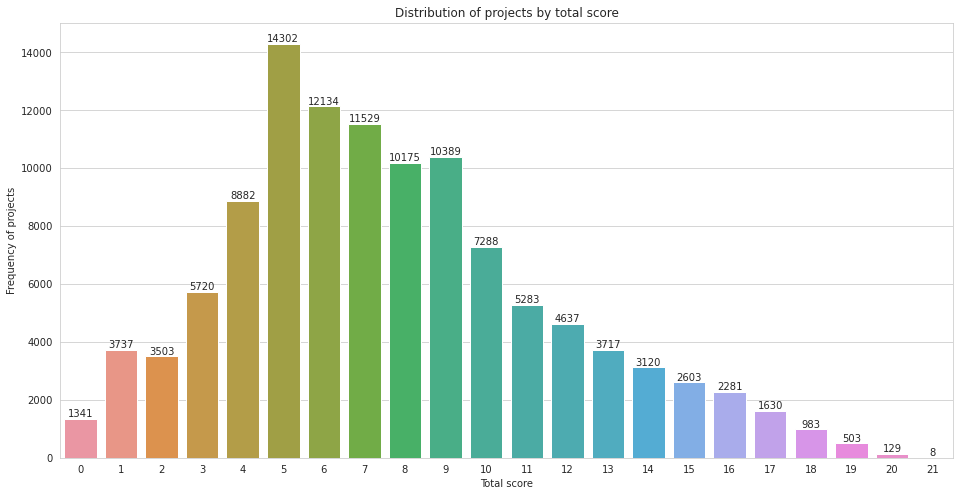
\includegraphics[bb=0 0 800 600, width=11cm, keepaspectratio]{img/frequency_total_score.png}
  	\caption{Distribución de proyectos de Snap! por puntuación total.}\label{fig:total}
\end{figure}

Como se aprecia en la figura~\ref{fig:total} existe una mayor concentración de los proyectos entre las puntuaciones totales de 4 y 10 puntos. La moda se localiza en los 5 puntos. La distribución de frecuencias absolutas es representada a partir del diagrama de barras.

%%%%%%%%%%%%%%%%%%%%%%%%%%%%%%%%%%%%%%%%%%%%%%%%%%%%%%%%%%%%%%%%%%%%%%%%%%%%%%%%
%%%%%%%%%%%%%%%%%%%%%%%%%%%%%%%%%%%%%%%%%%%%%%%%%%%%%%%%%%%%%%%%%%%%%%%%%%%%%%%%
% CONCLUSIONES %
%%%%%%%%%%%%%%%%%%%%%%%%%%%%%%%%%%%%%%%%%%%%%%%%%%%%%%%%%%%%%%%%%%%%%%%%%%%%%%%%

\cleardoublepage
\chapter{Conclusiones}
\label{chap:conclusiones}


\section{Consecución de objetivos}
\label{sec:consecucion-objetivos}

Esta sección es la sección espejo de las dos primeras del capítulo de objetivos, donde se planteaba el objetivo general y se elaboraban los específicos.

Es aquí donde hay que debatir qué se ha conseguido y qué no. 
Cuando algo no se ha conseguido, se ha de justificar, en términos de qué problemas se han encontrado y qué medidas se han tomado para mitigar esos problemas.

Y si has llegado hasta aquí, siempre es bueno pasarle el corrector ortográfico, que las erratas quedan fatal en la memoria final.
Para eso, en Linux tenemos aspell, que se ejecuta de la siguiente manera desde la línea de \emph{shell}:

\begin{verbatim}
  aspell --lang=es_ES -c memoria.tex
\end{verbatim}

\section{Aplicación de lo aprendido}
\label{sec:aplicacion}

Aquí viene lo que has aprendido durante el Grado/Máster y que has aplicado en el TFG /TFM. 
Una buena idea es poner las asignaturas más relacionadas y comentar en un párrafo los conocimientos y habilidades puestos en práctica.

\begin{enumerate}
  \item a
  \item b
\end{enumerate}


\section{Lecciones aprendidas}
\label{sec:lecciones_aprendidas}

Aquí viene lo que has aprendido en el Trabajo Fin de Grado/Máster.

\begin{enumerate}
  \item Aquí viene uno.
  \item Aquí viene otro.
\end{enumerate}


\section{Trabajos futuros}
\label{sec:trabajos_futuros}

Ningún proyecto ni software se termina, así que aquí vienen ideas y funcionalidades que estaría bien tener implementadas en el futuro.

Es un apartado que sirve para dar ideas de cara a futuros TFGs/TFMs.


%%%%%%%%%%%%%%%%%%%%%%%%%%%%%%%%%%%%%%%%%%%%%%%%%%%%%%%%%%%%%%%%%%%%%%%%%%%%%%%%
%%%%%%%%%%%%%%%%%%%%%%%%%%%%%%%%%%%%%%%%%%%%%%%%%%%%%%%%%%%%%%%%%%%%%%%%%%%%%%%%
% APÉNDICE(S) %
%%%%%%%%%%%%%%%%%%%%%%%%%%%%%%%%%%%%%%%%%%%%%%%%%%%%%%%%%%%%%%%%%%%%%%%%%%%%%%%%

\cleardoublepage
\appendix
\chapter{Manual de usuario}
\label{app:manual}

Esto es un apéndice.
Si has creado una aplicación, siempre viene bien tener un manual de usuario.
Pues ponlo aquí.

%%%%%%%%%%%%%%%%%%%%%%%%%%%%%%%%%%%%%%%%%%%%%%%%%%%%%%%%%%%%%%%%%%%%%%%%%%%%%%%%
%%%%%%%%%%%%%%%%%%%%%%%%%%%%%%%%%%%%%%%%%%%%%%%%%%%%%%%%%%%%%%%%%%%%%%%%%%%%%%%%
% BIBLIOGRAFIA %
%%%%%%%%%%%%%%%%%%%%%%%%%%%%%%%%%%%%%%%%%%%%%%%%%%%%%%%%%%%%%%%%%%%%%%%%%%%%%%%%

\cleardoublepage

% Las siguientes dos instrucciones es todo lo que necesitas
% para incluir las citas en la memoria
\bibliographystyle{abbrv}
\bibliography{memoria}  % memoria.bib es el nombre del fichero que contiene
% las referencias bibliográficas. Abre ese fichero y mira el formato que tiene,
% que se conoce como BibTeX. Hay muchos sitios que exportan referencias en
% formato BibTeX. Prueba a buscar en http://scholar.google.com por referencias
% y verás que lo puedes hacer de manera sencilla.
% Más información: 
% http://texblog.org/2014/04/22/using-google-scholar-to-download-bibtex-citations/

\end{document}
